\title{Tutorial for the TextureReconstruction application}
\author{Alexandre Morgand, France}
\date{\today}

\documentclass[12pt]{article}

\usepackage{hyperref}
\usepackage{subfigure}
\usepackage{graphicx}

\begin{document}
\maketitle

\section{Introduction}
This document describes a quick tutorial to the usage of the TextureReconstruction application.
The tutorial is divided in three components:
\begin{itemize}
    \item Camera calibration
    \item Reconstruction process of the texture of a planar surface (for now)
    \item Visualization of the reconstructed texture
\end{itemize}


\section{Camera Calibration}
\label{sec:calib}
In this section, we detailed an example of camera calibration in our application.
\subsection{Image loading}
From a couple of images of the OpenCV calibration grid\footnote{https://docs.opencv.org/2.4/\_downloads/pattern.png} taken from the camera that will be used for the texture reconstruction, the distortion parameters will be estimated as long as the intrinsic parameters as described 
\href{https://docs.opencv.org/2.4/doc/tutorials/calib3d/camera\_calibration/camera\_calibration.html}{here}. A couple of images used with a webcam camera are illustrated in figure \ref{fig:calib_webcam}.
\begin{figure}[!ht]
    \centering
    \subfigure[]
    {
	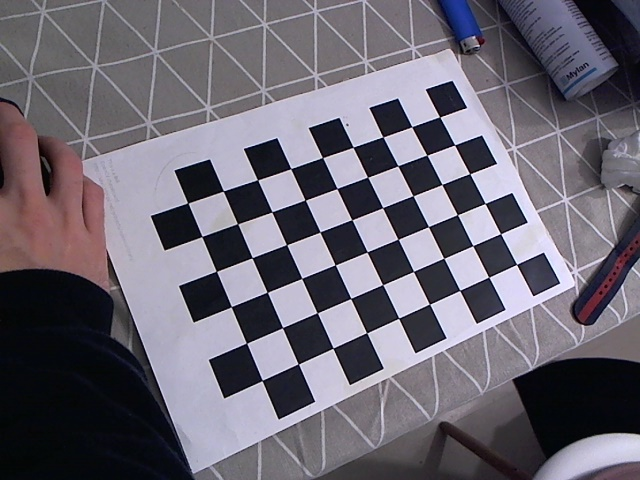
\includegraphics[width=0.45\linewidth]{img/im1.jpg}
    }
    \subfigure[]
    {
	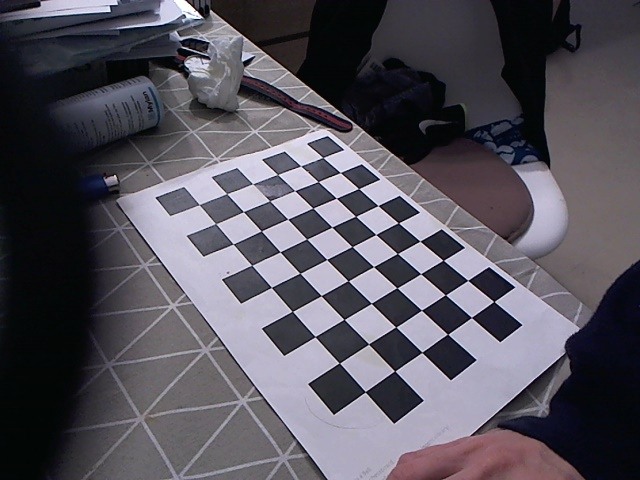
\includegraphics[width=0.45\linewidth]{img/im2.jpg}
    }
\caption{Webcam images of an OpenCV calibration grid.}
\label{fig:calib_webcam}
\end{figure}
To load the images, click on the \textbf{Load Images} button and select several of your images. 
\subsection{Calibration process}
After loading the images, click on the \textbf{Calibrate} button which is enabled once the loading is done. You will find in the top-left window the distorted image and its undistorted version in the top-right window. You can use the slider to iterate through the loaded images.
A complete illustrated of the UI is illustrated in figure \ref{fig:calibration}.

\begin{figure}[!ht]
    \centering
	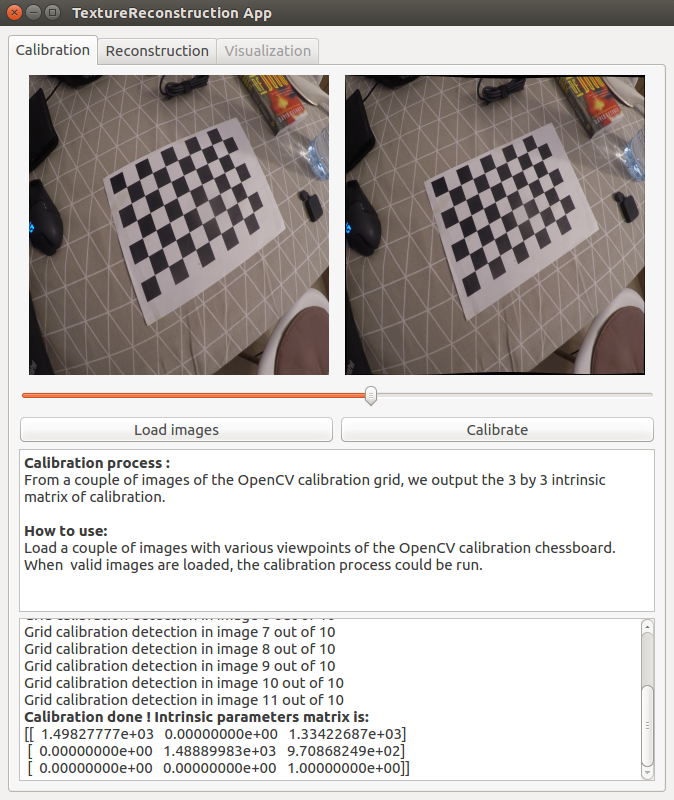
\includegraphics[width=\linewidth]{img/calibrated}
\caption{Screenshot of the UI after one camera calibration.}
\label{fig:calibration}
\end{figure}

\subsection{Recommendations}
For the calibration to be accurate, please follow these recommandations:
\begin{itemize}
    \item Be sure to use images where the calibration grid is clearly visible
    \item Use at least five images with various angles of view. The application will not perform the calibration otherwise
    \item If your images are really big, the calibration process could take more time. Be patient :) 
\end{itemize}

\section{Texture Reconstruction}
\label{sec:texture}
\subsection{Image loading}
From a couple of images of a planar object taken from the camera used for the calibration, we will reconstruct a texture from a planar surface.
To load the images, click on the \textbf{Load Images} button and select several of your images. 
 A first initialization step is done on a new window after the loading step by clicking on the corners of the object (exactly 4 for the moment). This process is illustrated in figure \ref{fig:initialization}

A couple of images used with a webcam camera are illustrated in figure \ref{fig:recon_webcam}.
\begin{figure}[!ht]
    \centering
    \subfigure[]
    {
	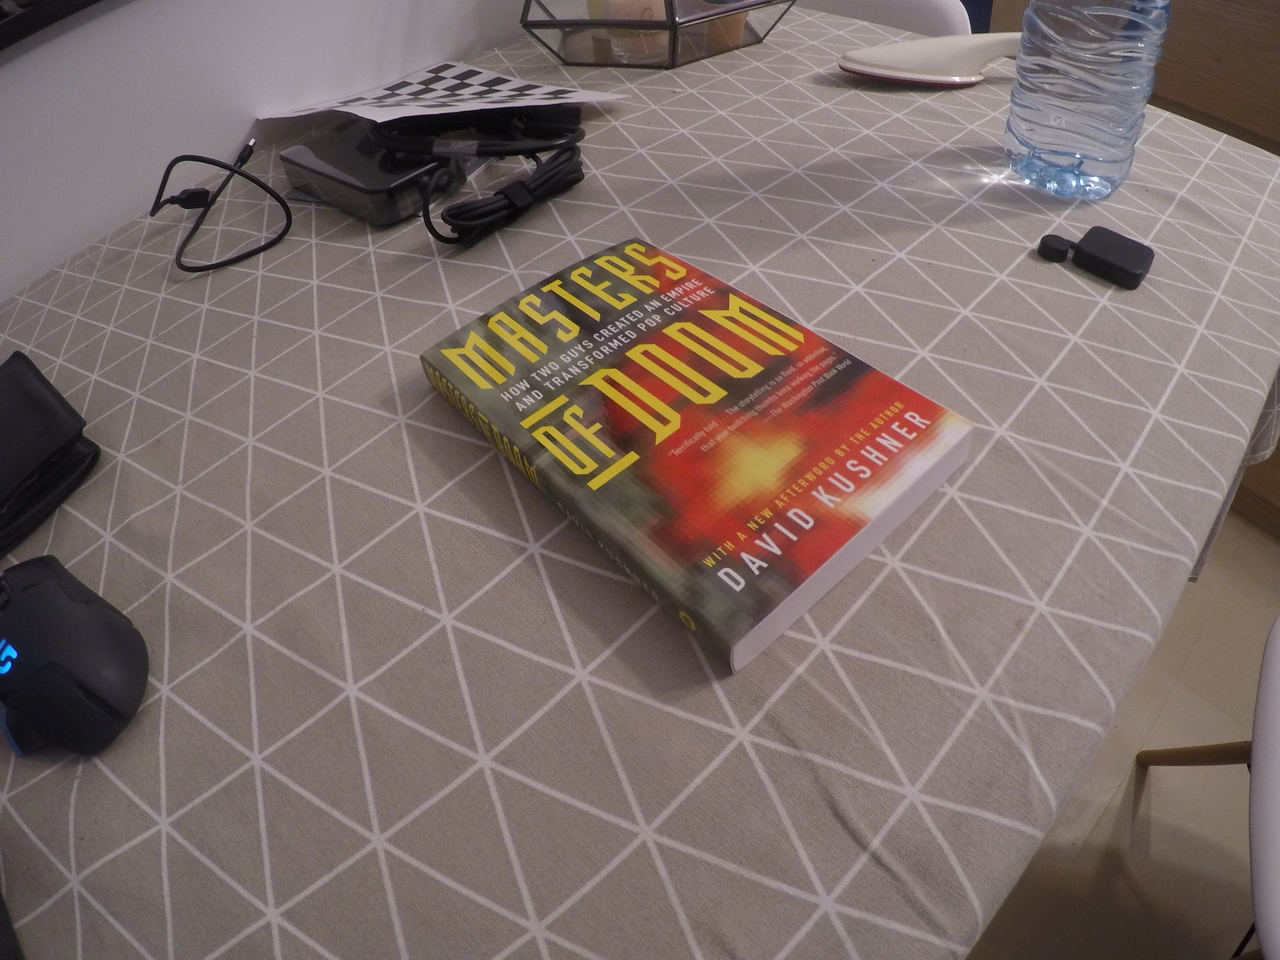
\includegraphics[width=0.3\linewidth]{img/recon1.jpg}
    }
    \subfigure[]
    {
	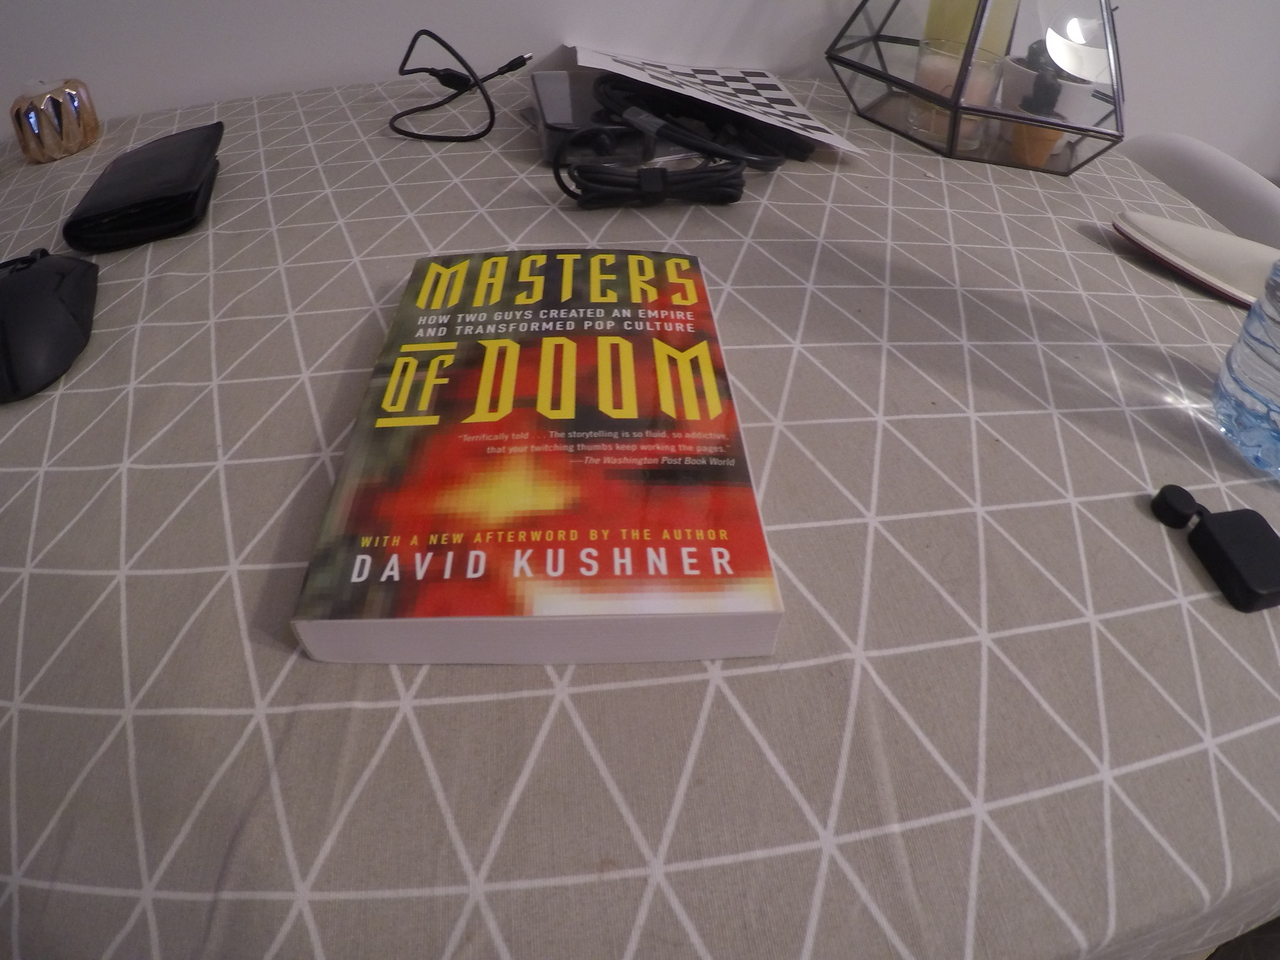
\includegraphics[width=0.3\linewidth]{img/recon2.jpg}
    }
    \subfigure[]
    {
	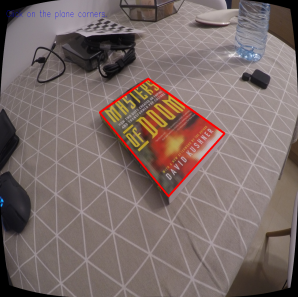
\includegraphics[width=0.3\linewidth]{img/init.PNG}
	\label{fig:initialization}
    }
\caption{(a) and (b) show images used for the reconstruction. In (c), we show the initialization process where the user click the corners of the planar texture.}
\label{fig:recon_webcam}
\end{figure}

\subsection{Image alignment}
After loading the images, click on the \textbf{Align Images} button which is enabled once the loading is done. You will find in the top-left window the align images and the reconstructed texture in the top-right window. You can use the slider to iterate through the loaded images.
\begin{figure}[!ht]
    \centering
	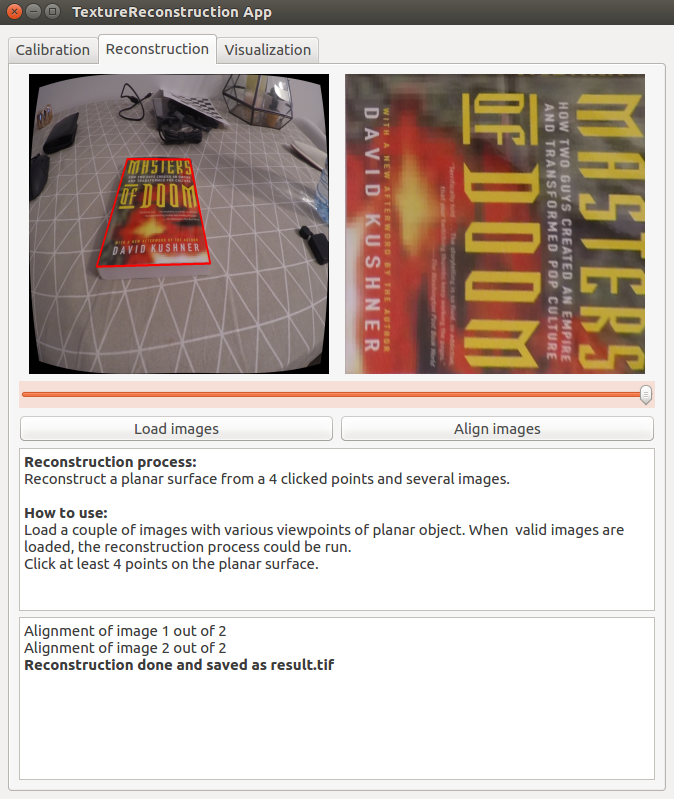
\includegraphics[width=0.8\linewidth]{img/reconstructed.PNG}
\caption{Screenshot of the UI after the reconstruction process.}
\label{fig:ui_init}
\end{figure}
The reconstructed texture will be saved as a tiff image \textbf{result.tiff}.

\subsection{Recommendations}
For the reconstruction process to be accurate, please follow these recommandations:
\begin{itemize}
    \item Be sure to use images where the object is clearly visible
    \item For the moment, we only reconstruct texture from planar surfaces with one image.
\end{itemize}

\section{Visualization Step}
\label{sec:vizu}
In the current version, this step is using an OSL shader applied to the reconstructed texture. To run the shader, click on the \textbf{Compile \& Run Shader} button. 
\subsection{Shader editing}
On the left window, you can edit directly your shader. If you want to apply the shader to the reconstructed texture, be sure to use the \textbf{result.tiff} as the input image.

\subsection{Vizualisation}

The visualization process in the UI is illustrated in figure \ref{fig:visu}.
\begin{figure}[!ht]
    \centering
	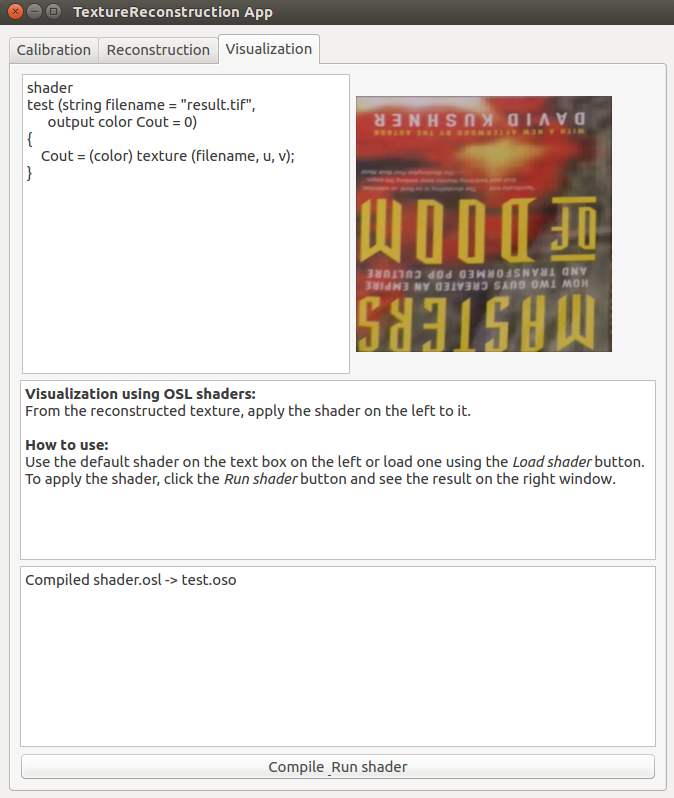
\includegraphics[width=0.8\linewidth]{img/visu.PNG}
\caption{Screenshot of the UI after the visualization.}
\label{fig:visu}
\end{figure}

\end{document}
